\section{Exceptional Interprocedural Control Flow Graphs}
\begin{frame}{Breakdown of Contribution}
  \begin{outline}[enumerate] % Don't think this environment works with <+-> directly
    \1<+-> \alert{Formal abstract model} of \gls{eh} \gls{abi} functions
    \1<+-> \alert{Algorithm} using model for \gls{cfr}
    \1<+-> \alert{Validation} of the model
    \1<+-> \alert{Evaluation} showing scalability and increased coverage
  \end{outline}
\end{frame}

\subsection{Example}
\begin{frame}{Returning to Example}
  \centering
  \tikzstyle{backdraw}=[< draw] % Had to reenable bEnd1's ability to draw outgoing edges here as setting it on the edge itself didn't work.
  % Trying to use \only/\uncover/etc. with the graph paths directly doesn't work so need to mess with the styles
  \only<1>{
    \tikzstyle{unwind}=[draw=none]
    \tikzstyle{backdraw}=[]
  }
  \only<-2>{\tikzstyle{good}=[]}
  \only<-3>{\tikzstyle{bad}=[]}
  \begin{tikzpicture}
    \graph[
      grow down=1.25cm,
      branch right=1.5cm,
      nodes={draw,ellipse,font=\ttfamily}
    ]{
      foo -> fEnd1/""[ret],
      foo -> "" -> {fEnd1, fEnd2/""[ret]}, % more compact this way
      foo'[landing] -> fEnd'/""[ret],

      bar -> {b1/"", bEnd1/""[ret,< draw=none]} -> {b2/"", bEnd2/""[ret]},
      b2 -> {bar[> bend left], bEnd2},
      b1 -> bEnd2, % necessary due to group/chain interactions
      bar'[landing] -> bEnd'/""[ret],

      {[grow down=1.25cm, branch right=1.5cm]
        {main[circle], catch[landing]} -> {
          callSite/""[diamond],
          ""[at=(0:-.5)],
          ""[ret, bad, at=(0:-1), < draw=none]
        } -> ""[ret,good],
      };

      callSite ->[interproc] foo;
      callSite ->[interproc] bar;

      fEnd1 ->[interproc] callSite;
      bEnd2 ->[interproc] callSite;

      fEnd2 ->[unwind] foo'; fEnd' ->[unwind] catch;
      bEnd1[backdraw] ->[unwind] bar'; bEnd' ->[unwind] catch;
    };
  \end{tikzpicture}
  \vfill
  \begin{tabular}{rl}
    \uncover<2->{\textcolor{red}{Red dashes} & \alert{unwinding} edges \\}
    \uncover<3->{\textcolor{green}{Green triangle} & successful termination \\}
    \uncover<4->{\textcolor{red}{Red triangle} & exceptional termination}
  \end{tabular}
\end{frame}

\begin{frame}{State of the Art}
  \begin{outline}
    \1 Existing tools do not model binary-level exceptional control flow!
    \begin{center}
      
\includegraphics[width=1cm]{GHIDRA_1}
      \hspace{1cm}
      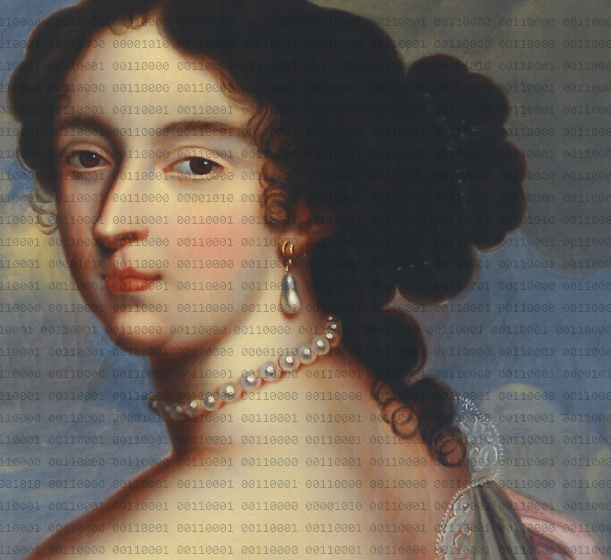
\includegraphics[width=1cm]{ida}
      \hspace{1cm}
      
\includegraphics[width=1cm]{ninja}
    \end{center}
    \1 Closest: IECFGs, which analyze \gls{cpp} source
  \end{outline}
\end{frame}

\subsection{Formulation}
\begin{frame}{Basics of State}
  \begin{outline}
    \1 Focused on \alert{exceptional state} and \alert{function calls}
    \1 Leaves out parts that can be overapproximated
      \2 Produced stack only contains return addresses!
    \1 Also requires static components from binary such as the \alert{landing pad table ($\landingpadtable$)}
      \2 Encodes unwinding destinations for ranges of addresses
  \end{outline}
\end{frame}

\begin{frame}{Generation}{What's the special bit?}
  \begin{outline}[enumerate]
    \1<+-> Extract $\landingpadtable$ from binary
    \1<+-> \alert{Symbolically execute} the binary
      \2<+-> Start from \glsxtrfull{ip} with initial \alert{symbolic state}
      \2<+-> Dissassemble instruction at that \gls{ip}
      \2<+-> Transform current state (including \gls{ip}) based on semantics of instruction (adds edge(s) to \gls{eicfg})
      \2<+-> Repeat with resulting state(s) until termination conditions encountered
    \1<+-> \alert{During 2.3, when encountering exceptional \gls{abi} calls, model them!}
  \end{outline}
\end{frame}

\begin{frame}{Modeling Exceptional \Glsxtrshort{abi} Calls}{Specification source: \citeurl{cxxEhAbi}}
  \begin{block}{\inlineasm{__cxa_throw}}
    \begin{outline}[enumerate]
      \1<+-> If current \gls{ip} is in $\landingpadtable$:
        \2<+-> Jump to target and stop unwinding
        \2<+-> Add corresponding edge to \gls{eicfg}
      \1<+-> Otherwise, unwind:
        \2<+-> Pop off current function call stack frame
        \2<+-> Jump to that frame's stored return address
        \2<+-> Add corresponding edge to \gls{eicfg}
      \1<+-> Repeat until no more stack frames are available, then terminate (\alert{unhandled exception})
    \end{outline}
  \end{block}
\end{frame}

\subsection{Validation}
\begin{frame}{How to check abstract semantics versus concrete?}
  \centering
  Compare to \alert<+>{real-world} executions of the functions being modeled!
  \vfill
  \begin{equation}
    \alert<+>{\sigma\absTransition\sigma'}
    \land
    \alert<+>{\gamma(\sigma)\concTransition s'}
    \implies
    \alert<+>{\alpha(s')=\sigma'}
    \label{eq:validation}
  \end{equation}
  \vfill
  Requires real-world \alert<+>{crafted programs} for the functions though\dots
\end{frame}

\begin{frame}{Process}
  \begin{outline}[enumerate]
    \1<+-> \alert{Fuzz} the \alert{abstract} states to get set of \alert{inputs} (we generated \glssymbol{fuzz-count})
    \1<+-> Execute abstract function models to get abstract \alert{outputs}
    \1<+-> \alert{Concretize}, inject abstract inputs into crafted programs using \alert{test harness} (\gls{gdb} used to set breakpoints, overwrite and view concrete program state)
    \1<+-> Check \alert{abstracted} \alert{concrete} outputs against abstract outputs for corresponding inputs
  \end{outline}
\end{frame}

\begin{frame}{Results}
  \centering
      \begin{tabular}{lccccccc}
    \toprule
    \thead{Rule} & \thead{$\rip$} & \thead{in/out regs} & \thead{$\handlerCount$} & \thead{$\uncaught$} & \thead{$\mathsf{handlerSwitchValue}$} & \thead{$\caught$} \\
    \midrule
    \inlineasm{__cxa_throw} & \checked & \checked & \checked & \checked && \\
    \inlineasm{__cxa_begin_catch} & \checked & \checked & \checked & \checked & \checked & \\
    \alert{\inlineasm{__cxa_end_catch}} & \checked & n/a & \checked & \checked & \checked & Partial \\
    \alert{\inlineasm{__cxa_rethrow}} & \checked & \checked & \checked & \checked && Partial \\
    \alert{\inlineasm{_Unwind_Resume}} && \checked & \checked & \checked & \checked & \\
    \bottomrule
  \end{tabular}
\end{frame}

\begin{frame}{Results of Validation}{Some Discoveries}
  \begin{outline}
      \1 Concrete implementation of \inlineasm{__cxa_begin_catch} takes absolute value of negative handler counts supplied to it before incrementing that value
      \1 \inlineasm{__cxa_rethrow} decreases $\handlerCount$ magnitude by one, then inverts sign; if the magnitude is 0, it is unchanged
  \end{outline}
\end{frame}

\subsection{Evaluation}
\begin{frame}{Case Studies}
  \begin{outline}
    \1<+-> Tested \glssymbol{total-bins} programs from a variety of sources
      \2 Publicly available \gls{nasa} tools
      \2 Programs and libraries from \gls{xen} hypervisor
      \2 Various printing-related and document type conversion tools available on Linux
      \2 Miscellaneous other programs
    \1<+-> Combination of \gls{c}, \gls{cpp}, even \gls{fortran}
    \1<+-> Special handling:
      \2<+-> Treated all function symbol addresses in binaries as potential starting \glspl{ip}
      \2<+-> Did two runs, one with \gls{eh} support, one without; compared results
  \end{outline}
\end{frame}

\begin{frame}{Statistics Summarized}
  \centering
  \begin{tabular}{l
      r% S[table-format=3]
      S[table-format=7] % total inst count
      S[table-format=7]
      S[table-format=4]
      S[table-format=4]
      S[table-format=6.0]
      |
      S[table-format=5] % inst coverage differential
    }
    \toprule
    & \multicolumn{6}{c}{\thead{Absolute Numbers}} & {\thead{Baseline\\Comparison}} \\
    \midrule
     & {\thead{Bin Count}} & {\thead{Covered\\Insts}} & {\thead{Unwind\\Edges}} & {\thead{Unique\\Throws}} & {\thead{Caught\\Throws}} & {\thead{Time/\si\second}} & {\thead{Inst Diff}} \\
    \midrule
    Totals & \glssymbol{eicfg-bin-success}/341 & 4715806 & 1269649 & 3350 & 2356 & 105809 & 45032 \\
    \bottomrule
  \end{tabular}
\end{frame}

\begin{frame}{Discussion and Limitations}
  \begin{columns}
    \column{.35\textwidth}
    \begin{block}{Uses}
      \begin{outline}
        \1 Strengthening static analyses
        \1 Improving decompilation
      \end{outline}
    \end{block}

    \pause
    \column{.55\textwidth}
    \begin{block}{Limitations}
      \begin{outline}
        \1 Contextuality for some indirections still an issue
        \1 No concurrency support here either
          \2 Thread-spawning functions treated as single-threaded
        \1 Even here not all indirections are resolvable
          \2 How to deal with that?
      \end{outline}
    \end{block}
  \end{columns}
\end{frame}
